\section{Architektur von Webanwendungen}\label{web_architecture} \thispagestyle{nomarkstyle}
Da es sich bei einem Online-Shop um eine Webanwendung handelt, ist es notwendig die allgemeine Architektur von solchen Anwendungen, sowie die unterschiedlichen Technologien, die eingesetzt werden können, zu analysieren.
Diese Information wird später wichtig um eine Architekturentscheidung passend zu den Anforderungen und Zielen treffen zu können.

Moderne Webanwendungen werden heutzutage überwiegend nach der Client-Server-Architektur aufgebaut. Anders als bei den rein serverbasierten Ansätzen, wird im Client-Server-Ansatz nicht eine komplette Seite im Server generiert und dem Client übermittelt.
Stattdessen bekommt der Client initial eine Seite mit wenig Daten geliefert, die per asynchronen Aufrufen vom Server geholt werden \cite{Saternos2014}.

Ein Modell dieser Architektur ist die Three-Tier-Architektur. Hierbei ist die Anwendung in drei logische Schichten unterteilt \cite{Techopedia2017}:
\begin{itemize}
	\item \textit{Tier 1: Präsentationsschicht.} Ist für die Darstellung der Daten und allgemein der Benutzerschnittstelle verantwortlich.
	\item \textit{Tier 2: Anwendungsschicht.} Auch Businesslogik-Schicht genannt, kontrolliert diese Schicht die eigentliche Funktionalität der Anwendung.
	\item \textit{Tier 3: Datenschicht.} Enthält die physischen Daten, üblicherweise in einer separaten Datenbank.
\end{itemize}

\autoref{fig:three-tier} veranschaulicht diese Unterteilung der logischen Komponenten im Zusammenhang mit der Trennung von Client und Server. %TODO Bild an die richtige Stelle bringen

\begin{figure}[ht!]
	\centering
	\includegraphics[width=\linewidth]{bilder/kap2/three-tier}
	\caption{Drei-Schichten-Modell der Client-Server-Architektur \cite{Conallen2000}}
	\label{fig:three-tier}
\end{figure}

\subsection{Serverseite}
Ein wichtiger Punkt der serverseitigen Architektur ist die Auswahl einer passenden Programmiersprache. Zu den Aufgaben solcher Programmiersprachen gehören hauptsächlich das Entgegennehmen und Beantworten von Anfragen des Clients, sowie die Kommunikation mit der Datenbank (falls vorhanden).
Welche Sprache hierfür gewählt wird bestimmt auch die Frameworks und weitere Technologien, die entsprechend zur Verfügung stehen. Im Folgenden sind einige der beliebtesten Sprachen für die Server-Programmierung, sowie jeweils die Frameworks, welche oft im Rahmen der Web-Entwicklung damit verwendet werden aufgelistet \cite{School2016}:

\begin{itemize}
	\item \textbf{C\#}. Objektorientiert, von Microsoft für die .NET Common Language Runtime entwickelt. \textit{Framework: ASP.NET}
	\item \textbf{Java.} Objektorientiert, universell einsetzbar und robust. \textit{Framework: Spring}
	\item \textbf{Node.js.} Entstand durch die wachsende Popularität von JavaScript in der Web-Programmierung. Hierbei wird die JavaScript-Syntax für Clients auch im Server benutzt. \textit{Frameworks: Express und Hapi}
	\item \textbf{PHP.} Wurde von Anfang an für die Entwicklung dynamischer Webanwendungen konzipiert und ist die verbreitetste Programmiersprache in diesem Bereich. \textit{Frameworks: Laravel und Symfony}
	\item \textbf{Ruby.} Gewann deutlich Popularität nach der Veröffentlichung des Frameworks Ruby on Rails. \textit{Framework: Ruby on Rails}
\end{itemize}

\subsubsection{Webserver}
Die Aufgabe eines Webservers ist es, die Inhalte einer Webseite per \acs{HTTP} an den Client zu liefern. In der Regel handelt es sich hierbei um statische Inhalte, also \acs{HTML}-Dateien, Bilder aber auch dynamisch generierte Dateien.
Für die dynamische Erzeugung von Dateien können Webserver Skriptsprachen wie Perl, PHP, ASP oder JSP unterstützen.

Die verbreitetsten Webserver-Produkte sind Apache \acs{HTTP} Server, Microsoft Internet Information Server (\acs{ISS}) und nginx \cite{Rouse2012}.

\subsubsection{Applikationsserver}
Ein Applikationsserver liefert, konkret im Bereich der Webanwendungen, die notwendige Businesslogik um dynamische Inhalte generieren zu können, sowie andere Funktionalitäten bereitzustellen. Dieser Server ist direkt an den Webserver angeschlossen und fängt die Anfragen nach dynamischem Inhalt ab.
Diese werden dann zum Beispiel mit einer Kombination aus Templates, laufenden Programmen und Datenbankzugriffen erzeugt. \cite{ITWissen.info2013}

\subsubsection{Datenbank}
Für die Datenhaltung in einer Webanwendung werden fast immer Datenbanken verwendet, um Inhalte unabhängig von der Anwendung persistent speichern zu können.
Dabei werden meist relationale oder \acs{NoSQL}-Datenbanken eingesetzt.

Relationale Datenbanken bilden in ihrem Datenmodell die Beziehungen zwischen den einzelnen Datensätzen ab.
Als Entitäten bezeichnet, werden logisch unabhängige Datensätze in jeweils eigenen Tabellen gespeichert. Jeder Datensatz ist dabei in einer eigenen Zeile gespeichert und die Tabellenspalten stellen die einzelnen Attribute dar.
Verweise auf andere Entitäten für die Abbildung der Beziehungen werden durch sogenannte Fremdschlüssel-Spalten realisiert, die als Wert einen bestimmten Datensatz einer anderen Entität referenzieren können.
Die am meisten verwendeten Produkte relationaler Datenbanken sind Oracle Database, MySQL, Microsoft SQL Server, PostgreSQL und DB2. \cite{solidIT2017}

\acs{NoSQL}-Datenbanken sind die häufigste Alternative zu den relationalen Lösungen. Der Name ist ein Akronym für \enquote{Not only SQL} und spielt damit auf die Beschränkungen der verbreitetsten Datenbanksprache \acs{SQL} relationaler Modelle an.
Unter dieser Kategorisierung gibt es verschiedene Modelle. Folgend sind die wichtigsten Datenmodelle mit je einem Beispiel \cite{solidIT2017a}:

\begin{itemize}
\item\textbf{Dokumentenorientierte Datenbanken.} MongoDB
\item\textbf{Key-Value-Datenbanken.} Redis
\item\textbf{Graphdatenbanken.} Neo4j
\item\textbf{Spaltenorientierte Datenbanken.} Apache Cassandra
\end{itemize}

\subsubsection{ORM}
Unter dem Object Relational Mapping, kurz \acs{ORM}, versteht man die Zuordnung der Repräsentation von Objekten in der verwendeten Programmiersprache zu der dafür vorgesehenen Datenstruktur in der relationalen Datenbank.
Diese Aufgabe benötigt sowohl eine technische Lösung zur Anbindung und Ansteuerung der Datenbank aus der Anwendung, als auch eine logische für die richtige Zuordnung von Objekten auf Entitäten-Tabellen und Objekt-Attributen auf deren Spalten.
Für die Anbindung der Datenbank gibt es je nach eingesetzter Programmiersprache und Datenbank-Technologie spezielle Tools, auf die an dieser Stelle nicht näher eingegangen werden soll.
Zum Zweck des Mappings, also der logischen Zuordnung, gibt es Hilfe in Form von Frameworks, die es ebenfalls für die verschiedenen zugrunde liegenden Technologien gibt.
Die wichtigsten Vertreter sind hier das Entity Framework für .NET-Sprachen und Hibernate für Java.

\subsection{Clientseite}
Die wichtigsten clientseitigen Webtechnologien sind schon seit einigen Jahren HTML, CSS und JavaScript. Hierbei sind HTML und CSS Technologien für die Darstellung der Webseite und JavaScript allgemein für die clientseitige Programmierung zuständig\cite{Thattil2016}. 

\subsubsection{JavaScript Erweiterungen}
Ein wichtiger Wendepunkt in der Geschichte von JavaScript war die Einführung von \acs{AJAX} (\enquote{Asynchronous JavaScript and XML}). Durch AJAX wurde es möglich, asynchrone Anfragen zum Server durchzuführen, um Teile einer Seite zu verändern ohne sie komplett neu laden zu müssen. Ein großer Vorteil davon ist die erhöhte Reaktionsgeschwindigkeit der Weboberfläche, da diese nicht durch die Anfragen blockiert wird.

Kurze Zeit später kamen die sogenannten JavaScript Document Object Model (\acs{DOM}) Libraries wie \textit{jQuery} dazu. Diese Bibliotheken fügten zahlreiche nützliche Funktionalitäten zur einfachen Manipulation der DOM und zur Implementierung von AJAX-Aufrufen mit deutlich weniger Code\cite{Fink2014}.

\subsubsection{Arten von Webanwendungen}\label{web_types}
Die bereits erwähnten Verbesserungen an JavaScript, aber auch an HTML mit der Veröffentlichung von HTML5, brachten mit sich neue Techniken mit denen neuartige Anwendungen aufgebaut werden konnten. Single Page Applications (\acs{SPA}s) sind eine Art von Webanwendung die in diesem Rahmen erschien. In den nächsten Abschnitten werden zum Vergleich die traditionelle Webanwendungen, sowie die moderne Single Page Applications näher beschrieben.

\paragraph{Traditionelle Webanwendungen}$\;$ \\
Eine traditionelle Webanwendung generiert die dargestellte Webseite immer wieder neu wenn eine beliebige HTTP Anfrage eingeht. Das gilt demnach nicht nur für den initialen Aufruf der Webseite sondern auch zum Beispiel für das Senden eines ausgefüllten Formulars. Die im Server erzeugte HTML-Seite wird als Antwort zum Client gesendet, was dort wiederum eine Aktualisierung bewirkt. Bei einer Aktualisierung lädt der Browser die Seite neu und ersetzt dabei die ursprüngliche HTML durch die neue\cite{Fink2014}. \cref{fig:traditional-web} veranschaulicht diesen Ablauf.

\begin{figure}[ht!]
	\centering
	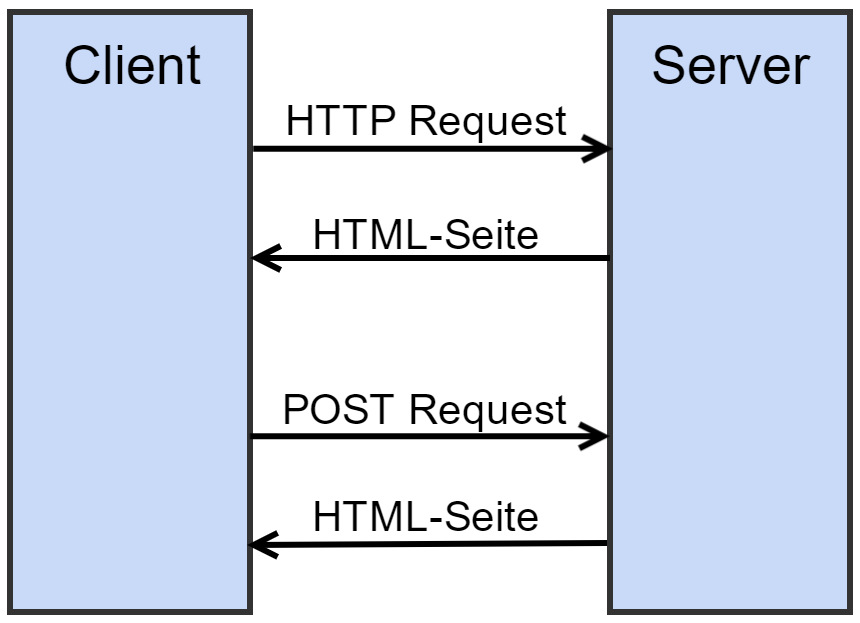
\includegraphics[width=0.5\linewidth]{bilder/kap2/trad_web}
	\caption{Lebenszyklus einer traditionellen Webanwendung}
	\label{fig:traditional-web}
\end{figure}

\paragraph{Single Page Applications}$\;$ \\
Wie auf \cref{fig:spa} zu erkennen ist, gibt es beim initialen Aufruf der Webseite keine Unterschiede zwischen traditionellen und Single Page Anwendungen. Bei allen weiteren Anfragen ist der Ablauf jedoch anders. Durch AJAX sind die Anwendungen in der Lage Anfragen an den Server zu senden, bei denen nur die notwendige Daten angefordert werden. Der Client erhält daraufhin eine Antwort, welche diese Daten enthält (üblicherweise im \acs{JSON}-Format). Sobald die Daten ankommen, kann der Client die HTML-Seite partiell anpassen, ganz ohne Neuladen des Browser-Fensters. Dieser Ablauf ist für alle Benutzerinteraktionen in der Anwendung gleich, selbst für die Navigation. Das macht die Antwortzeiten solcher Anwendungen sehr kurz, was eine sehr positive Auswirkung auf die Benutzerzufriedenheit hat.

\begin{figure}[ht!]
	\centering
	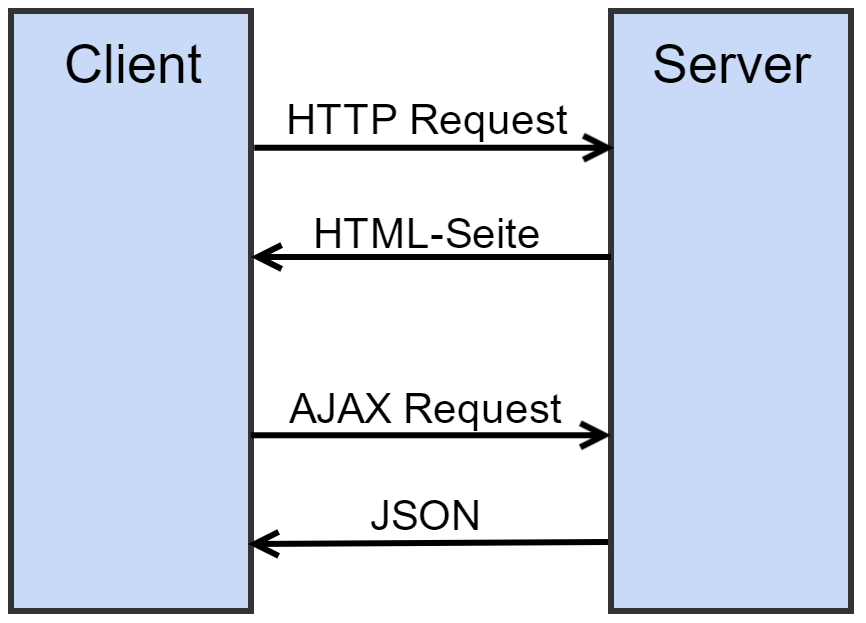
\includegraphics[width=0.5\linewidth]{bilder/kap2/spa}
	\caption{Lebenszyklus einer \acs{SPA}}
	\label{fig:spa}
\end{figure}






